%%%%%%%%%%%%%%%%%%%%%%%%%%%%%%%%%%%%%%%%%%%%%%%%%%%%%%%%%%%%%%%%%%%%%%%%%%%%%%%%%%%%%%%%%%%%%%%%%%%%%%%

\documentclass[prl,aps,11pt,superscriptaddress,floatfix]{revtex4-2} 
\usepackage{graphicx}
\usepackage{color} 
\usepackage{amsmath}
\usepackage{amssymb} 
\usepackage{natmove}
\usepackage{natbib}
\usepackage{hyperref} 
\usepackage{bm}

%%%%%%%%%%%%%%%%%%%%%%%%%%%%%%%%%%%%%%%%%%%%%%%%%%%%%%%%%%%%%%%%%%%%%%%%%%%%%%%%%%%%%%%%%%%%%%%%%%%%%%%

\begin{document}

\title{\huge On the Origin of Shrimpoluminescence }

\author{\large Tyler C. Sterling}
\email{ty.sterling@colorado.edu}
%\affiliation{Department of Physics, University of Colorado at Boulder, Boulder, Colorado 80309, USA}

\date{\today}

%\begin{abstract}
%    abstract
%\end{abstract}

\maketitle

%\listoffigures
%\listoftables
%\tableofcontents

%%%%%%%%%%%%%%%%%%%%%%%%%%%%%%%%%%%%%%%%%%%%%%%%%%%%%%%%%%%%%%%%%%%%%%%%%%%%%%%%%%%%%%%%%%%%%%%%%%%%%%%

\begin{figure}
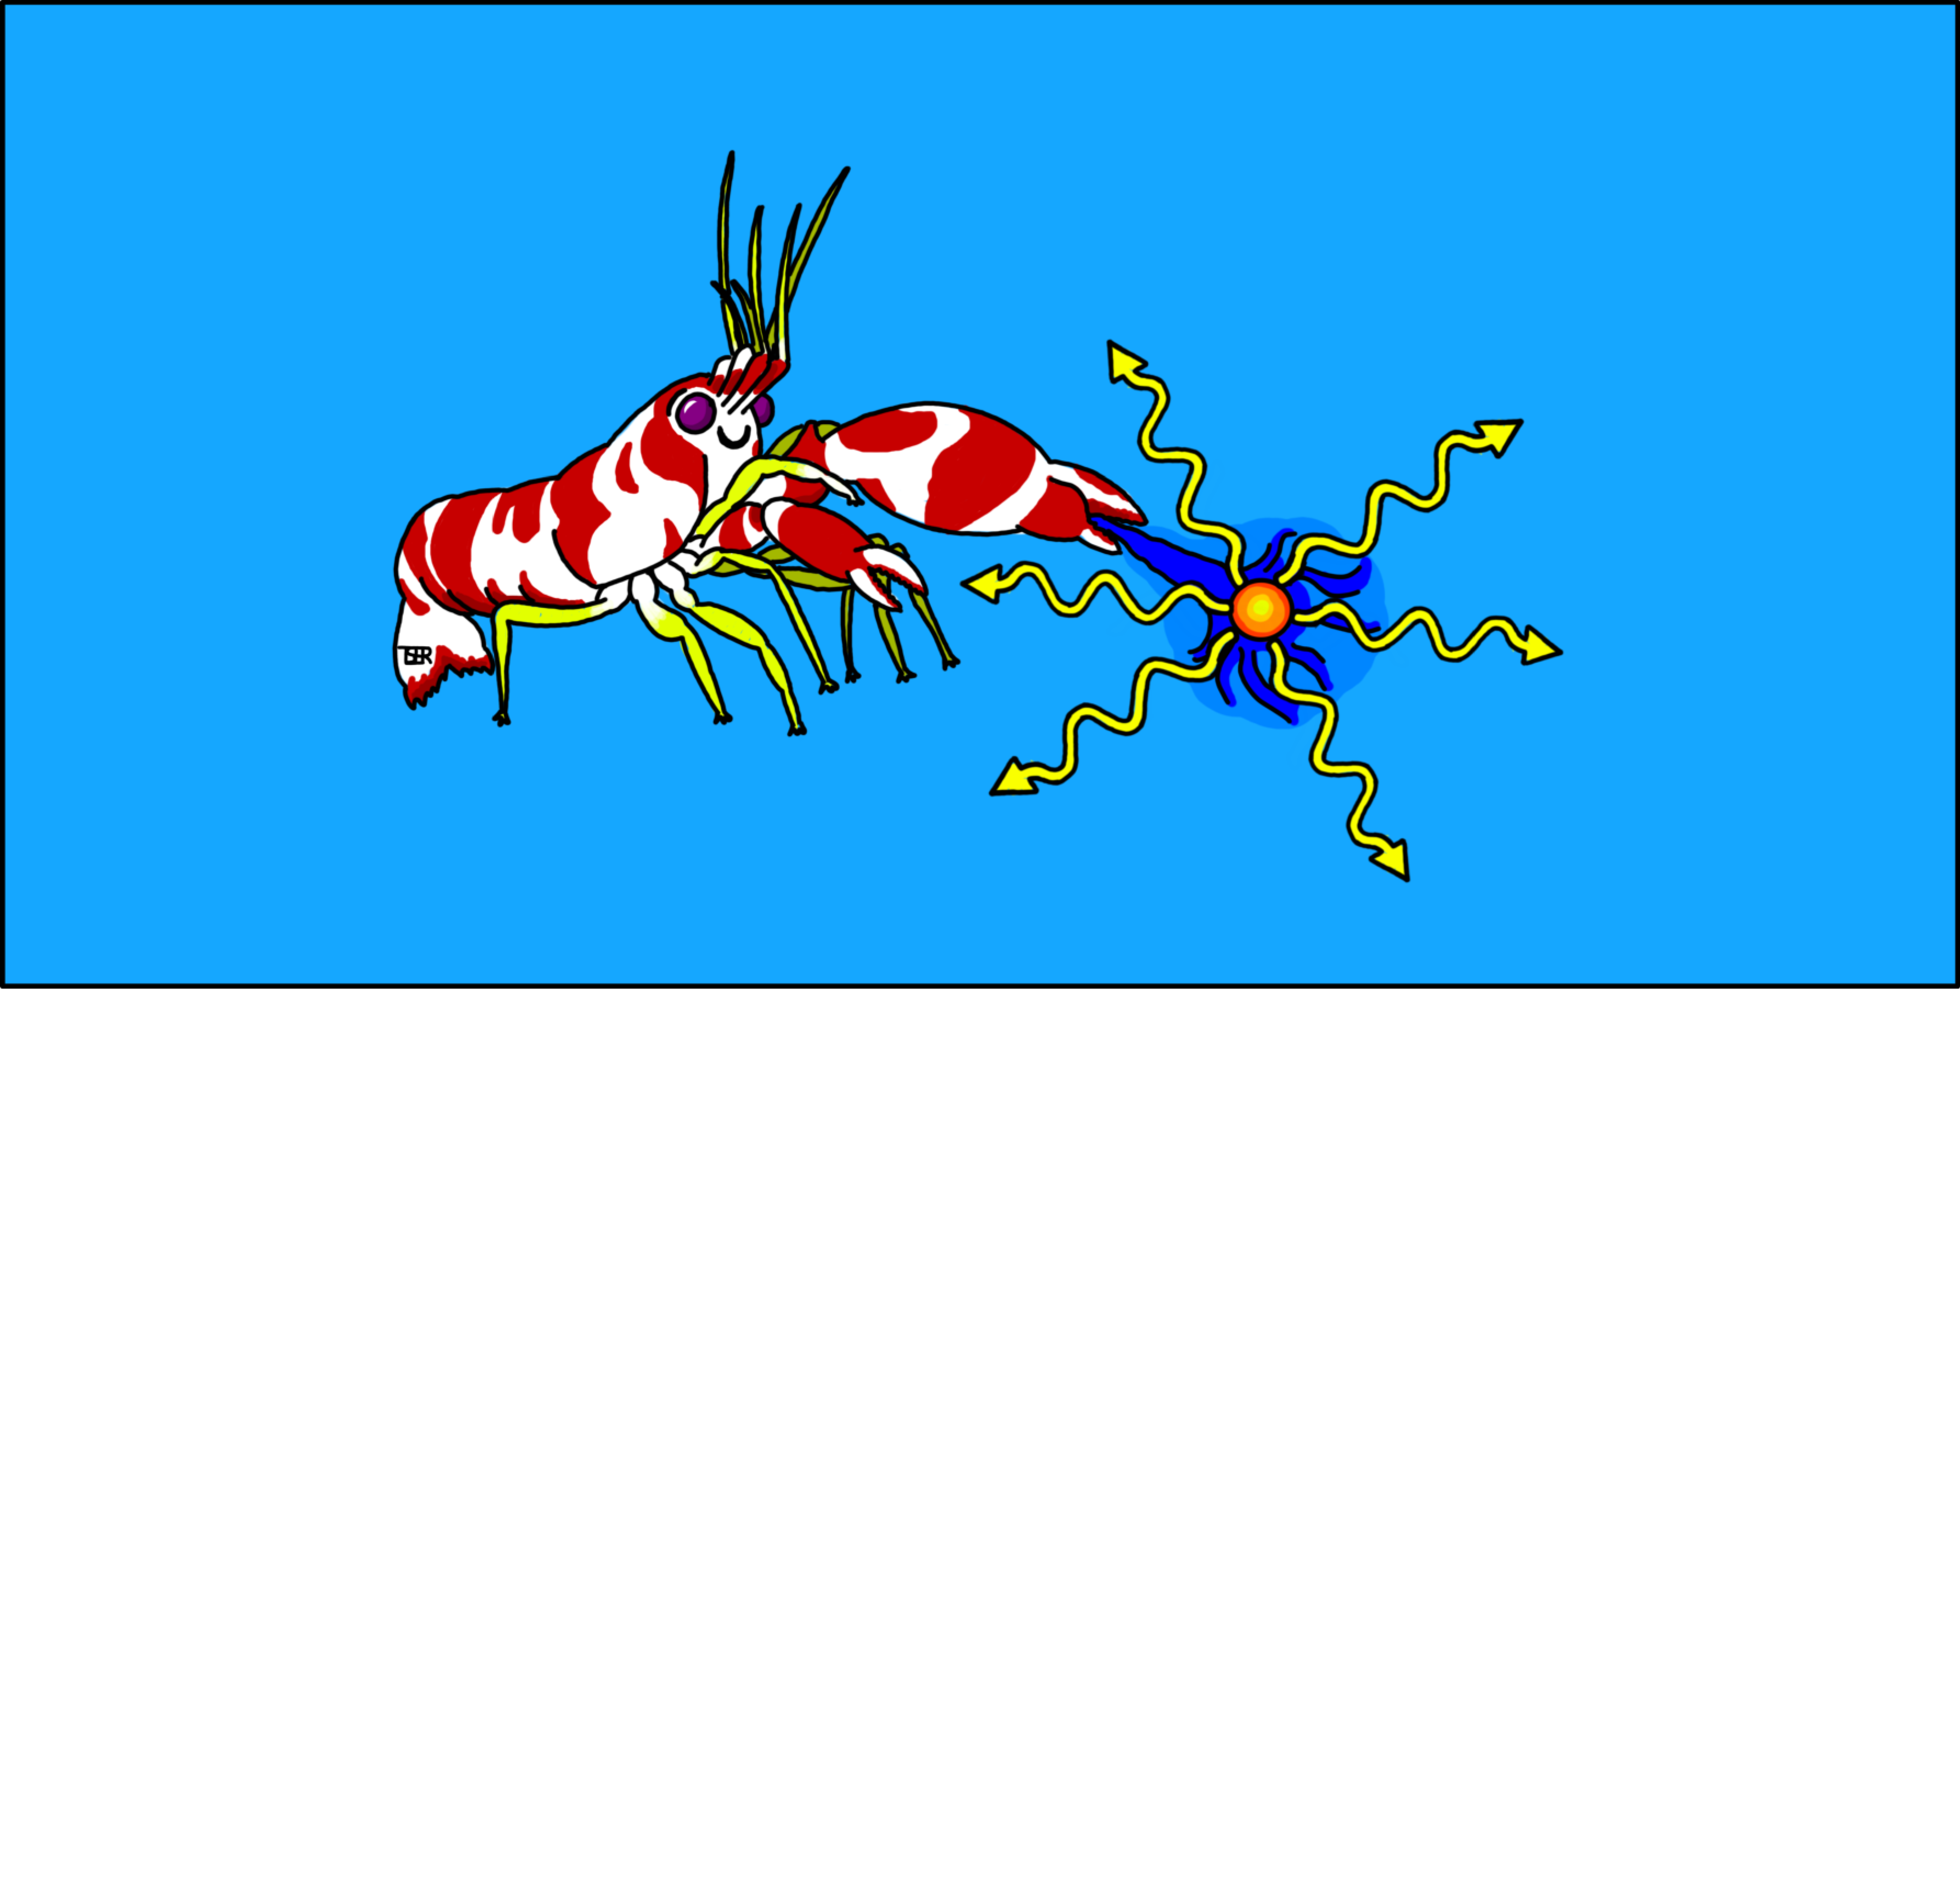
\includegraphics[width=1\linewidth]{../figs/shrimpy2.pdf}
%    \caption{}
\label{fig:shrimpy}
\end{figure}
 
\newpage

\section{Details...}
Pistol shrimp, like the red-banded pistol shrimp shown on the cover, are capabale of generating a jet of water with high enough velocity that a cavitation bubble forms behind it. When the bubble collpases, a powerful shock-wave is produced that can kill the shrimp's prey \cite{versluis2000snapping}. If the shrimp's prey had very sensitive eyes (and also weren't dead) they might notice a flash of light is also produced through an effect referred to as ``shrimpoluminescence" in the case of the pistol shrimp \cite{lohse2001snapping}, but more generally known as \emph{sonoluminescence}.

Sonoluminescence can be more precisely defined as the effect in which light is produced when an ultrasonically driven bubble collapses \cite{borisenok2020mechanisms}. Unlike the shrimp's method, laboratory techniques can produce stable, single bubbles that can be driven and collapsed with high precision. As such, quite a bit of effort has been spent studying \emph{single-bubble sonoluminescence} (SBSL) \cite{lohse2018bubble,brenner2002single}. Yet the physical origin of the light production has eluded understanding. There are two prevailing theories: (i) the effect is of a thermal origin and (ii) it is an electrical effect \cite{borisenok2020mechanisms}. The thermal argument is based on the observation that the temperature of the gas trapped in the bubble when light is emmited is $\sim$10000 K! \cite{flannigan2005plasma,lohse2018bubble} (for reference, the surface of the Sun is about 6000 K). It is beleived that thermal radiation (among other mechanisms) could be the source of the light. The electrical arguments are instead based on the belief that the collapsing bubble does not remain spherical: the asymmetrical shape of the bubble leads to the formations of \emph{jets} that cause non-Newtonian fracturing in the liquid \cite{prosperetti1997new}. There is subsequently a dielectric break-down at the fracture and the electrical spark is the source of the light. Along similar lines, it has been argued that the rapidly deforming bubble polarizes the water at the bubble's surface, leading to an (electric) polarization field. Assuming the thermal effects are also true, it was argued that free electrons from the ionized gas in the bubble enter the polarized water layer and form a plasma that emmits the light.

On the other hand, I can't ignore an ``alternative" theory which is actually what led me to this topic: a phenomenological theory based on quantum electrodynamics. This subject will get us pretty far afield but I will try to spend some time on this too because, well, it sounds interesting! In short, Schwinger \cite{schwinger1993casimir} and subsequently others \cite{liberati2000sonoluminescence,eberlein1996sonoluminescence} have argued that changes in the \emph{Casimir energy} due to changing the volume of a dielectric sphere can lead to production of photons. 

\section{About me}

My undergraduate degree is in manufacturing; I worked with industrial robots on manufacturing process optimization. I also completed a masters degree in materials science at CU before transferring into the physics PhD program. In the materials science program, I worked in the aerospace department using molecular dynamics to study (lattice) thermal conductivity in thermoelectrics. Now I work for Dmitry Reznik so my research is still focused on lattice-dynamics but my methods are based on computational electronic-structure theory (i.e DFT). We usually look at fancy materials like cuprates or magnets, but we also study energy materials like thermoelectrics and hybrid perovskites. The point is, none of this is even closely related to shrimpoluminscence. 

I plan to have fun writing this paper and I hope you will have fun reading it! 



%%%%%%%%%%%%%%%%%%%%%%%%%%%%%%%%%%%%%%%%%%%%%%%%%%%%%%%%%%%%%%%%%%%%%%%%%%%%%%%%%%%%%%%%%%%%%%%%%%%%%%%

\bibliography{../ref}

\end{document}
